\chapter{VivadoFPGA}

The Xilinx Vivado software can be downloaded from the Xilinx website\cite{54}.
Registration is required.

To install the software
\begin{verbatim}
  tar -zxf Xilinx_Vivado_SDK-WIN_2015.2_0626_1.tar.gz
  cd Xilinx_Vivado_SDK-WIN_2015.2_0626_1
  xsetup
  agree to licenses
  choose Vivado WebPACK
  choose Next
  choose Next (for destination directory)
  choose Install
  choose Get Free Licenses
  click Connect Now
  sign in
  choose all four Activation Based Licenses
  click Activeate Node-Locked License
  on the Generate Node License popup, click Next
  on the Review License Request, click Next
\end{verbatim}

In this part, we use the Vivado to do some simple implementation of
VHDl code, and try to run on the Altera's FPGA boards.

\begin{figure}[ht!]
\centering
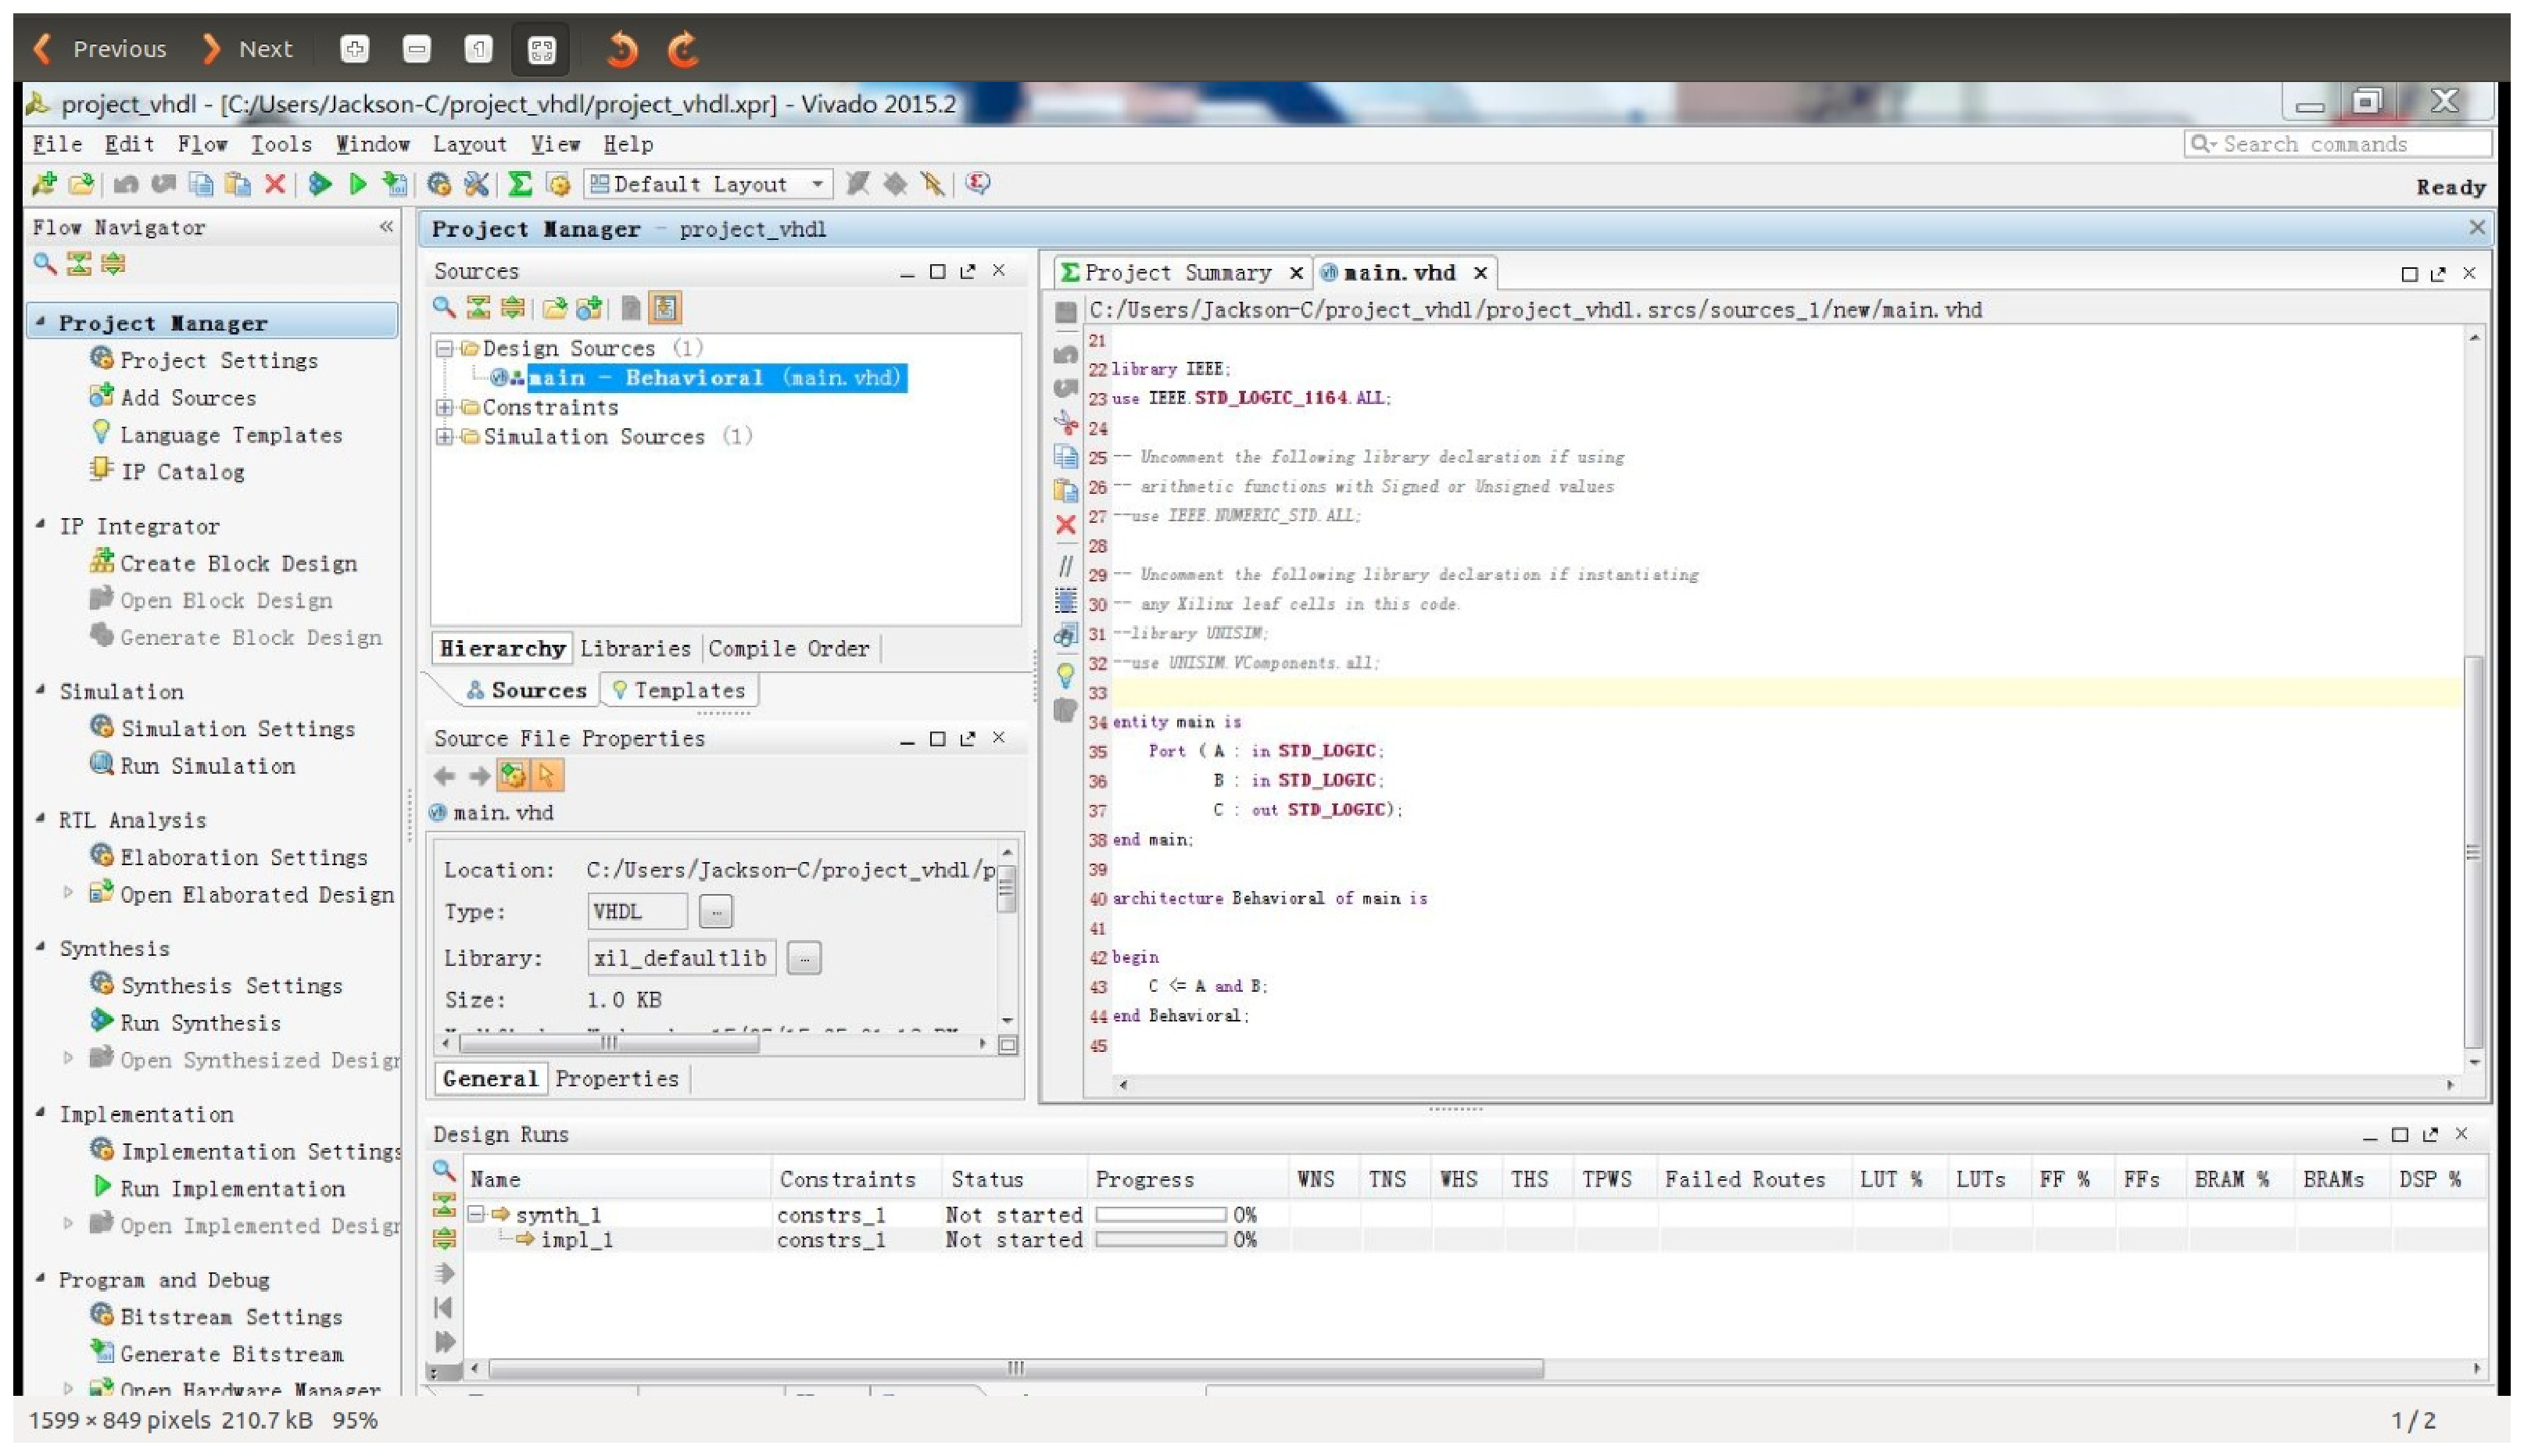
\includegraphics[scale=0.25]{eps/vivado1.eps}
\caption{The vivado1}
\label{vivado1}
\end{figure}

As can be seen in Figure~\ref{vivado1}, the code we use to illustrate
the vivado workflow is simple. two input signals A and B, one output
signal C. The transformation logic between them is: C $<=$ A and B.

The code:

\begin{chunk}{ANDvhdl}

library IEEE;
use IEEE.STD_LOGIC_1164.ALL;

entity main is
	For: (A:in STD_LOGIC;
		B:in STD_LOGIC;
		C:out STD_LOGIC);
end main;

architecture Behavioral of main is

begin
	C<=A and B;
end Behavioral;

\end{chunk}


\begin{figure}[ht!]
\centering
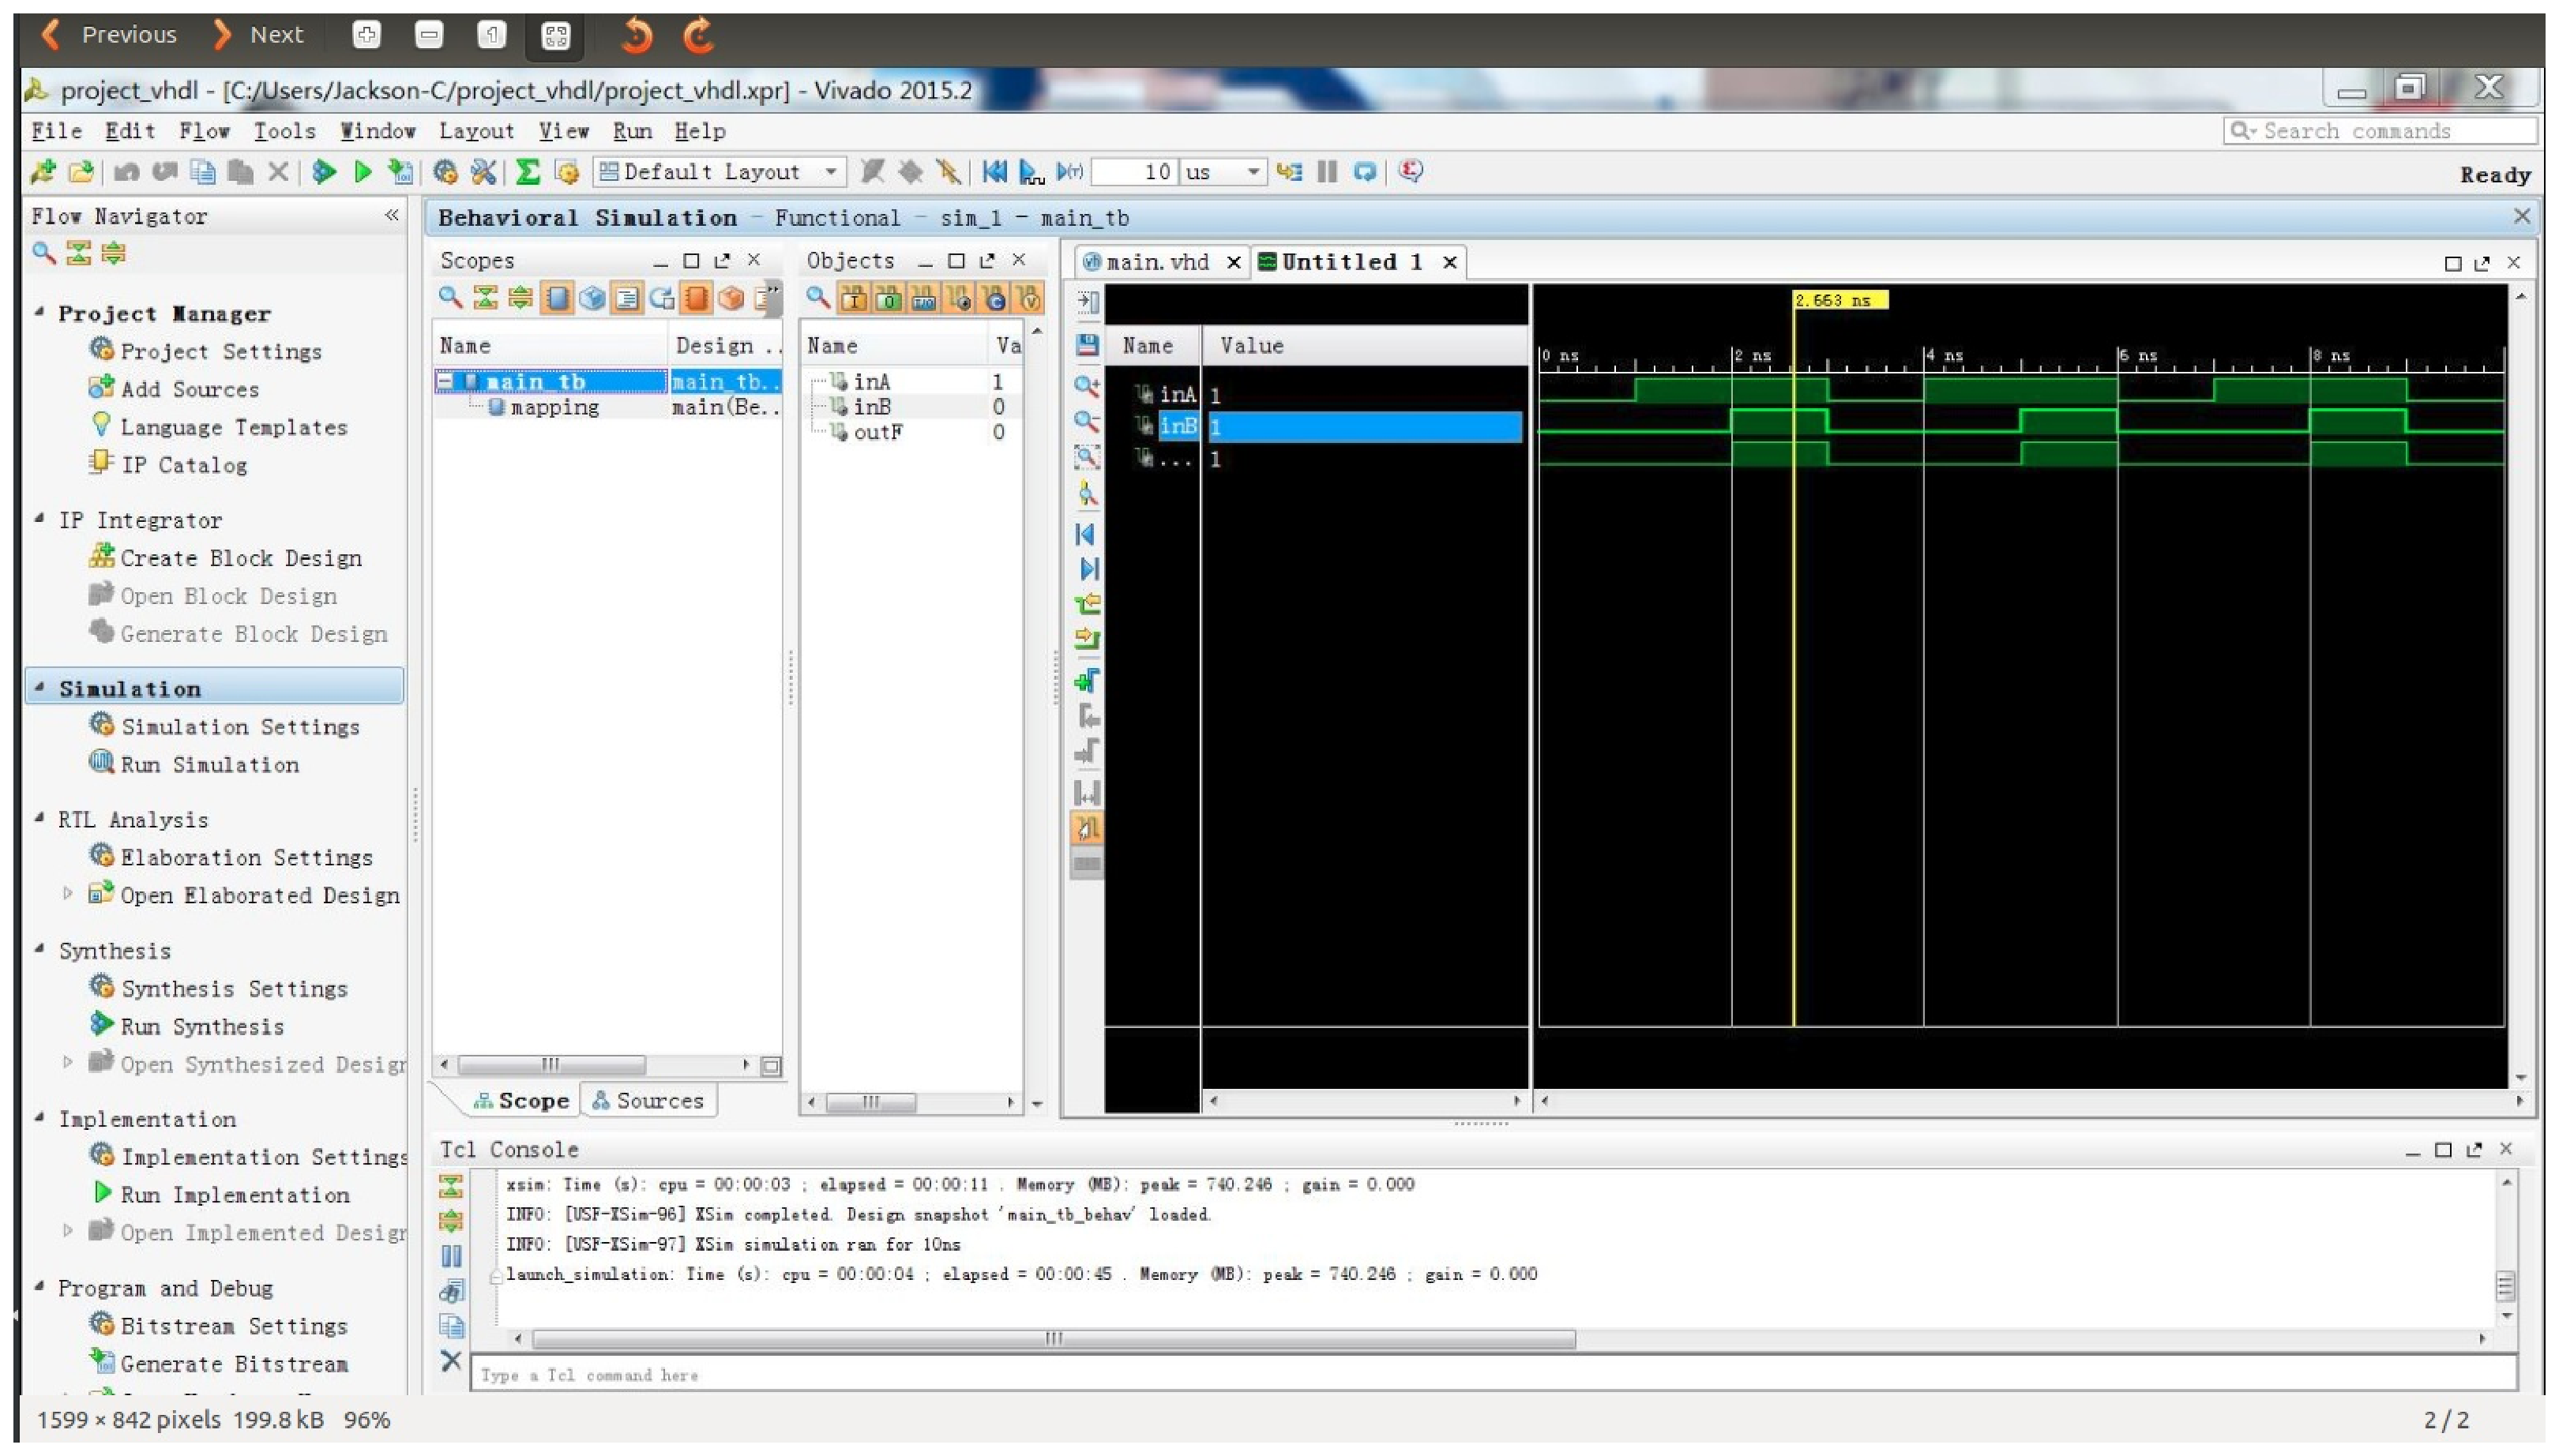
\includegraphics[scale=0.25]{eps/vivado2.eps}
\caption{The vivado2}
\label{vivado2}
\end{figure}

As can be seen in Figure~\ref{vivado2}, we can find the waveform after
simulating the vhdl code we presented above and it's easy to see the
transformation logic behind the scenes.

Some Useful video links to use Vivado:


Vivado Design Flows Overview (v2013.1): From \cite{59}

This video briefly describes the Vivado Design workflow. There are two
Use Models:
\begin{enumerate}
\item Tcl scripted or GUI based use models
\begin{itemize}
\item Run entire flow manually using Vivado Tcl Shell commands or scripts
\item Run entire flow with the press of a button using the Vivado IDE
\end{itemize}
\item Batch compilation style flow or project based flow
\begin{itemize}
\item Manually manage all sources, design commands and configuration, and
reporting using Tcl commands and scripts (Non-Project Mode)
\item Create a Project infrastructure on disk to manage entire design
process and track status (Project Mode)
\end{itemize}
\end{enumerate}
And some other things to be mentioned:
\begin{enumerate}
\item IP-Centric System-level Design Integration
\begin{itemize}
\item Create IP subsystems with IP Integrator
\item Configure, validate and instantiate IP using the IP Catalog
\end{itemize}
\item System Design Entry through Hardware Validation Flows
\begin{itemize}
\item Advanced design, analysis and process management capabilities
\end{itemize}
\item Flexible Use Models
\begin{itemize}
\item Tcl accessible common data model throughout the flow
\item Project and compilation style flows
\item Support for third party software tools
\end{itemize}
\item Programming and Debugging Design in Hardware: From \cite{60}:\\
This video briefly explains and shows the steps to program and debug
in Hardware using Vivado:
\begin{enumerate}
\item Connecting to the hardware and programming the FPGA
\item Setting up the ILA debug core trigger and probe simple compare conditions
\item Arming the ILA debug core and capture data in the waveform window
\end{enumerate}
\item Logic Simulation: From \cite{61}:

This video shows how to simulate a design in Vivado IDE:
\begin{enumerate}
\item Simulation Settings
\item Launching Vivado Simulator
\item Waveform Viewer
\end{enumerate}
\end{enumerate}

And it lists some of the advantages that Vivado provides:
\begin{enumerate}
\item Easy to manage simulation sources and settings
\begin{itemize}
\item automatically compile and simulate sources
\end{itemize}
\item Fully integrated simulator
\begin{itemize}
\item powerful simulator engine (3x faster than ISE Simulator)
\item Common waveform viewer
\end{itemize}
\end{enumerate}

And that could be part of the reasons why we choose Vivado rather than ISE.

